

\chapter{Sprint 3}
\label{Sprint0}
\lhead{Chapter 9. \emph{Sprint 3}}

\section{Goal(s)}

The main goal of this sprint was the mid-term delivery of the report; this corresponded to
the second project's milestone M2. Furthermore, another important goal was the continued development
of the second prototype of the system which would feature HealthVault interoperability.

\section{Planning}

The plan consisted in an initial focus on report writing in order to receive as much
feedback as possibile on it. We understood that this was a good chance to receive
valuable feedback from a) the student advisor, b) the technical advisor, c) the customer.

After mid-term delivery we scheduled to do some system and application development.
%Also, we didn't want to fall behind schedule with system development so we planned some
%development as well

\section{Duration}

\begin{itemize}
\item Sprint start:  October, 7th
\item Milestone M2 (mid-term report delivery): October, 14th.
\item Sprint end: October, 20th
\end{itemize}

\section{Backlog}

\begin{itemize}
\item \textbf{M2 Mid-term report}:
	delivery of the mid-term report. Although this delivery was not graded we made an effort
	to produce as much documentation as possible in order to receive extensive feedback from
	1) the student advisor 2) the technical advisor 3) the customer.
\item \textbf{Project management}\newline
	This included:
	\begin{itemize}
		\item \textbf{Weekly startup meeting}: 
		\item \textbf{Meeting notes}:
			taking notes during meetings, reviewing of the notes.
		\item \textbf{Status reports}:
			for both week 41 and 42
		\item \textbf{Risk analysis}:
			updated on a weekly basis, so twice per sprint.
			%% The risk analisys was submitted to the supervisor and the customer.
		\item \textbf{Planning for the next iteration}:
			the project manager prepared a plan for the next iteration
			which would be illustrated and agreed upon on next iteration's startup meeting.
	\end{itemize}
	\item \textbf{Weekly meetings}: 
		meetings with both the customer and the supervisor. Beginning this sprint, we also
		had an internal meeting with our colleague in Oslo.
	\item \textbf{Application development}:
		continued development of the Android application.
	\item \textbf{System development}:
		we performed some studies on the different ways we could deploy the backend
		1) as a WAR file in a separate servlet container (Apache Tomcat) 2) as a Spring JAR file
		with embedded servlet support. Furthermore we continued development
	\item \textbf{}
	
\end{itemize}



69,Project management,,15,Done,100,emanuele,,,,"Plan next iteration	emanuele	Done
Meeting documents	SebZal	Done
Startup meeting (week 41)	Done

Status report (week 41)	emanuele	Todo
Status report (week 42)	emanuele	Done

Update risk analysis	emanuele	Done
Documentation review	emanuele	Todo"

62,Weekly meetings (week 41),"Meeting with the customer.
Meeting with the supervisor.
Internal meeting (once a week).",7,Done,200,"emanuele, Andersos, SebZal",,None,,

61,Report work (week 41),,25,Done,300,"emanuele, SebZal",,,,

68,Additional report work (week 41),Additional report work by Anders,10,Todo,400,Andersos,,,,

63, Weekly meetings (week 42),Meeting with the customer. Meeting with the supervisor. Internal meeting (once a week).,7,Todo,500,"emanuele, Andersos, SebZal",,None,,

13,M2 Mid-term report (14.10),Deliver the mid-term report.,?,Done,537,,,,,

64,System development,Front-end deployment as part of WAR file.,10,Done,575,"emanuele, SebZal",,,,

65,Application development,Continue weight application development.,10,Done,612,emanuele,,,,

70,Report work (week 42),,10,Done,631,"emanuele, SebZal",,,,

71,Additional report work (week 42),Additional report work by Anders,10,Todo,640,Andersos,,None,,

66,Testing,IP testing. Application testing. Integration system.,6,Done,650,"emanuele, Andersos, SebZal",,,,JUnit testing	Andersos	Todo



\section{Results and feedback}

This sprint proceeded smoothly.


\begin{figure}[H]
\centering
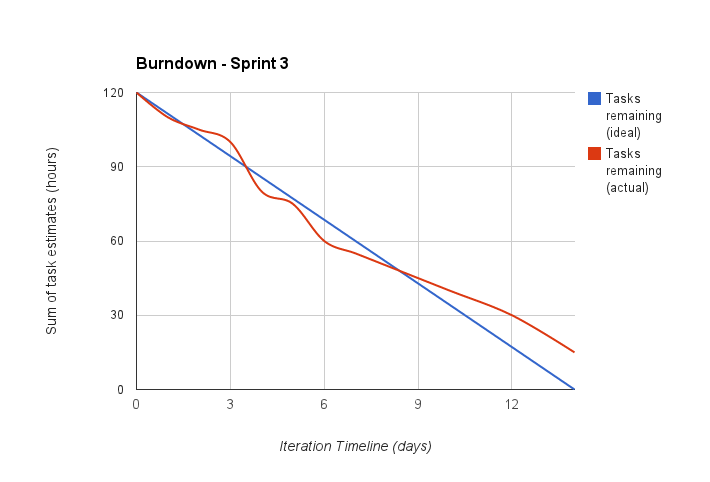
\includegraphics[scale=0.60]{../Figures/burndownSprint3.png}
\caption{Burndown chart Sprint 3}
\label{figure:burndownsprint3}
\end{figure}



\section{Evaluation}

